\documentclass[../main.tex]{subfiles}

\begin{document}

\section{Which Assessment Questions are the Most Difficult}
As learners engage in activities supported by a learning ecosystem, they will
experience learning content as well as assessment content. Assessments
are designed to measure the effectiveness of learning content and help
assess knowledge gained. It is possible that certain assessment questions
do not accurately represent the concepts contained within learning
content and this may be indicated by a majority of learners getting
the question wrong. It is also possible that the question accurately
represents the learning content but is very difficult. The following
algorithm will identify these types of questions but will not be able to deduce
why learners answer them incorrectly.

\subsection{Ideal Statements}
In order to accurately determine which assessment questions are the
most dificult, there are a few requirements of the data produced by a
LRP. They are as follows:
\begin{itemize}
\item statements describing a learner answering a question must report
  if the learner got the question correct or incorrect via $\$.result.success$
\item if it is possible to get partial credit on a question, the amount
  of credit should be reported within the statement
  \begin{itemize}
  \item the credit earned by the learner should be reported within \\ $\$.result.score.raw$
  \item the minimum and maximum possible credit amount should be
    reported within $\$.result.score.min$ and $\$.result.score.max$
    respectively
  \end{itemize}
\item If it is possible to get partial credit on a question, it must
  still be reported if the learner reached the threshold of success
  via $\$.result.success$
\item Statements describing a learner answering a question should
  contain activities of the type $cmi.interaction$
\item activities must be uniquely and consistently identified across
  all statements
\item Statements describing a learner answering a question
  should\footnote{\label{verbIRI} it is possible to use another verb iri but if another is
    used, that will need to be accounted for in data retrieval} use
  the verb $http://adlnet.gov/expapi/verbs/answered$
\end{itemize}

\subsection{Input Data Retrieval}
How to query an LRS via a GET request to the Statements Resource via
curl. The following section contains the appropriate parameters with
example values as well as the curl command necessary for making the request.\footnote{\label{refMoreLink} See footnote 1.}\footnote{\label{refnoZ} See footnote 2.}\footnote{\label{refallTime} See footnote 3.}

\begin{lstlisting}[frame=single]
  Verb = "verb=http://adlnet.gov/expapi/verbs/answered"

  Since = "since=2018-07-20T12:08:47Z"

  Until = "until=2018-07-21T12:08:47Z"

  Base = "https://example.endpoint/statements?"

  endpoint = Base + Verb + "&" + Since + "&" + Until

  Auth = Hash generated from basic auth

  S = curl -X GET -H "Authorization: Auth"
  -H "Content-Type: application/json"
  -H "X-Experience-API-Version: 1.0.3"
  Endpoint
\end{lstlisting}

\subsection{Statement Parameters to Utilize}

The statement parameter locations here are written in
\href{http://goessner.net/articles/JsonPath/}{JSONPath}. This notation
is also compatable with the xAPI Z notation due to the defined
hierarchy of components. Within the Z specifications, a variable name
will be used instead of the $\$$
\begin{itemize}
\item $\$.result.success$
\item $\$.object.id$
\end{itemize}

\subsection{2018 Pilot TLA Statement Problems}
The initial pilot test data supports this algorithm.
Given that the offical 2018 pilot test is scheduled to take place on July
27th, 2018, this section may require updates pending future data review.

\subsection{Summary}

\begin{enumerate}
\item Query an LRS via a \href{https://github.com/adlnet/xAPI-Spec/blob/master/xAPI-Communication.md#213-get-statements}{GET} request to the statements endpoint using the parameters verb, since and until
\item Filter the results to the set of statements where:
  \begin{itemize}
  \item $\$.result.success$ is false
  \end{itemize}
\item process the filtered data
  \begin{itemize}
  \item group by $\$.object.id$
  \item determine the count of each group
  \item create a collection of pairs = [$\$.object.id$, \#]
  \end{itemize}
\end{enumerate}

\subsection{Formal Specification}
\subsubsection{Basic Types}

$INCORRECT$ :== $\{false\}$

\subsubsection{System State}
\begin{schema}{MostDifficultAssessmentQuestions}
  Statements \\
  S_{all} : \finset_1 \\
  S_{incorrect},S_{grouped},S_{processed} : \finset \\
  \where
  S_{all} = statements \\
  S_{incorrect} \subseteq S_{all} \\
  S_{grouped} = \{groups : \seq_1 statement\} \\
  S_{processed} = \{pair : (id , \nat)\}
\end{schema}
\begin{itemize}
\item The set $S_{all}$ is a non-empty, finite set and is the
  component $statements$
\item The sets $S_{incorrect}$, $S_{grouped}$ and $S_{processed}$ are all finite sets
\item the set $S_{incorrect}$ is a subset of $S_{all}$ which may
  contain every value within $S_{all}$
\item the set $S_{grouped}$ is a finite set of objects $groups$ which
  are non-empty, finite sequences of the component $statement$
\item the set $S_{processed}$ is a finite set of pairs where each
  contains the component $id$ and a natural number
\end{itemize}
\subsubsection{Initial System State}

\begin{schema}{InitMostDifficultAssessmentQuestions}
  MostDifficultAssessmentQuestions \\
  \where
  S_{all} \not = \emptyset \\
  S_{incorrect} = \emptyset \\
  S_{grouped} = \emptyset \\
  S_{processed} = \emptyset
\end{schema}
\begin{itemize}
\item The set $S_{all}$ is a non-empty set
\item The sets $S_{incorrect}$ , $S_{grouped}$ and $S_{processed}$ are all initially empty
\end{itemize}

\subsubsection{Filter for Incorrect}

\begin{schema}{Incorrect}
  Statement \\
  incorrect : STATEMENT \pfun \finset \\
  s? : STATEMENT \\
  s! : \finset \\
  \where
  s? = statement \\
  s! = incorrect(s?) \\
  incorrect(s?) = \IF s?.result.success : INCORRECT \\\t4 \THEN s! =
  s? \\\t4 \ELSE s! = \emptyset
\end{schema}
\begin{itemize}
\item the schema $Incorrect$ introduces the function $incorrect$ which
  takes in the variable $s?$ and returns the variable $s!$
\item the variable $s?$ is the component $statement$
\item $s!$ is equal to $s?$ if $\$.result.success$ is of the type
  $INCORRECT$ otherwise $s!$ is an empty set
\end{itemize}

\begin{schema}{FilterForIncorrect}
  \Delta MostDifficultAssessmentQuestions \\
  Incorrect \\
  incorrects : \finset
  \where
  incorrects \subseteq S_{all} \\
  incorrects' = \{s : STATEMENT \,|\, incorrect(s) \not = \emptyset\} \\
  S_{incorrect}' = S_{incorrect} \cup incorrects'
\end{schema}
\begin{itemize}
\item the set $incorrects$ is a subset of $S_{all}$ which may contain
  every value within $S_{all}$
\item The set $incorrects'$ contains elements $s$ of type $STATEMENT$
  where $incorrect(s)$ is not an empty set
\item The updated set $S_{incorrect}'$ is the union of the previous
  state of $S_{incorrect}$ and $incorrects'$
\end{itemize}

\subsubsection{Processes Results}

\begin{schema}{GroupByActivityId}
  Statements \\
  g? : \finset \\
  g! : \finset \\
  group : \finset \fun \finset
  \where
  g? = statements \implies \{g : statement\} \\
  g! = group(g?) \\
  g! = \{groups : \seq_1 statement \,|\, \\ \t1
  \LET \seq_1 statement_{i}..statement_{j} == \seq_1 s_{i}..s_{j} @ \\\t1
  \forall s_{n} : s_{i}..s_{j} @ i \leq n \leq j @ s_{i}.object.id =
  s_{j}.object.id = s_{n}.object.id\} \\
\end{schema}
\begin{itemize}
\item The schema $GroupByActivityId$ introduces the function $group$
  which has the input of $g?$ and the output of $g!$
\item The input variable $g?$ is the component $statements$ which implies
  its a set of objects $g$ which are each a $statement$
\item the output variable $g!$ is a set of objects $groups$ which
  are each a non-empty, finite sequence of $statement$ where each
  member of the sequence $s_{i}..s_{j}$ has the same $\$.object.id$
\end{itemize}

\begin{schema}{CountPerGroup}
  Statement \\
  c? : \seq_1 statement \\
  c! : \nat \\
  count : \seq_1 statement \fun \nat
  \where
  c! = count(c?) \\
  c! \geq 1 \\
  count(c?) = \forall c_{n}? : \langle c?_{i}..c?_{j} \rangle @ i \leq n \leq j \land i
  = 0 @ \\\t3  \exists_1 \, c! : \nat @  \IF n = i \THEN c! = n + 1 \ELSE c!
  = j + 1

\end{schema}
\begin{itemize}
\item The schema $CountPerGroup$ introduces the function $count$
  which has the input of $c?$ and the output of $c!$
\item The input variable $c?$ is a non-empty, finite sequence in which each element is
  a $statement$
\item The function $count$ reads: for all elements $c?_{n}$ within the
  sequence $\langle c?_{i}..c?_{j} \rangle$, such that $n$ is greater than or
  equal to $i$ and less than or equal to $j$, $i$ is
  equal to zero and there exits a number $c!$ which is equal to $n +
  1$ (when $n = i \implies n = 0$) or equal to $n$
\end{itemize}

\begin{schema}{AggregateQuestionStatements}
  \Delta MostDifficultAssessmentQuestions \\
  FilterForIncorrect \\
  GroupByActivityId \\
  CountPerGroup \\
  grouped, processed : \finset \\
  \where
  grouped = \emptyset \\
  grouped' = group(S_{incorrect}) \\
  S_{grouped}' = S_{grouped} \cup grouped' \\
  processed \subseteq S_{grouped}' \\
  processed' = \{p : (id, \nat) \,|\, \\\t3 \LET
  \{\langle processed_{i}\rangle..\langle processed_{j}\rangle\} == \{g_{i}..g_{j}\} @ \\\t3
  i \leq n \leq j @ \forall g_{n} : g_{i}..g_{j} @ \exists \, p_{n} : p_{i}..p_{j} @ \\\t3
  first~p_{n} = head~g_{n}.object.id \, \land second~p_{n} =
  count(g_{n}) \\
  S_{processed}' = S_{processed} \cup processed'
\end{schema}
\begin{itemize}
\item The schema $AggregateQuestionStatements$ introduces the variables
  $grouped$ and $processed$
\item $grouped$ starts as an empty set but then becomes $grouped'$
  which is the output of applying the function $group$ to the set of statements
  $S_{incorrect}$ created by the opperation $FilterForIncorrect$
\item $grouped'$ is a set of sequences. The elements of those
  sequences are statements which all have the same
  $statement.object.id$

\item The set $S_{grouped}$ is updated to the set $S_{grouped}'$ which
  is the union of $S_{grouped}$ and $grouped'$
\item the variable $processed$ is a subset of $S_{grouped}'$ which can
  contain every value within $S_{grouped}'$
\item the variable $processed$ is updated to be the variable
  $processed'$ which is a set of objects $p$ which are ordered pairs
  of the component $id$ and a natural number. $p$ is defined as:
  \begin{itemize}
  \item for all sequences $g_{i}..g_{j}$ within the set $processed$,
    there exists an ordered pair $p_{n}$ such that:
    \begin{itemize}
    \item the first element of $p_{n}$ is equal to the $object.id$ of the first
      statement within the sequence $g_{n}$.
    \item The second element of $p_{n}$ is equal to the value returned
      when $g_{n}$ is passed to the function $count$.
    \end{itemize}
  \end{itemize}
\item The set $S_{processed}'$ is the union of the sets
  $S_{processed}$ and $processed'$
\end{itemize}

\subsubsection{Sequence of Operations}

$ProcessedQuestions \defs FilterForIncorrect \semi
AggregateQuestionStatements$

\begin{itemize}
\item The schema $ProcessedQuestions$ is the sequential composition
  of operation schemas $FilterForIncorrect$ and
  $AggregateQuestionStatements$
\item $FilterForIncorrect$ happens before $AggregateQuestionStatements$
\end{itemize}

\subsubsection{Return}

\begin{schema}{ReturnAggregate}
  \Xi MostDifficultAssessmentQuestions \\
  ProcessedQuestions \\
  S_{processed}! : \finset
  \where
  S_{processed}! = S_{processed}
\end{schema}
\begin{itemize}
\item The returned variable $S_{processed}!$ is equal to the current
  state of variable $S_{processed}$ after the operations
  $FilterForIncorrect$ and \\ $AggregateQuestionStatements$
\end{itemize}

\subsection{Pseudocode}

\begin{algorithm}[H]
  \SetAlgoLined
  \KwIn{$S_{all}$, $displayN$}
  \KwResult{$display''$}
  \emph{context = \{\}}\;
  \emph{display = []}\;
  \While{$S_{all} \not = \emptyset$}
  {\ForEach{$s \in S_{all}$}
    {\eIf{$s.result.success$ = $INCORRECT$}
      {\bf do \\
        $S_{incorrect}' \leftarrow s \cup S_{incorrect}$\;
        $S_{all}' \leftarrow S_{all} \setminus s$\;
        recur $S_{all}', S_{incorrect}'$\;}
      {\bf do \\
        $S_{all}' \leftarrow S_{all} \setminus s$\;
        recur $S_{all}'$}}}
  \While{$S_{incorrect}' \not = \emptyset$}
  {\ForEach{$si \in S_{incorrect}'$}
    {$id \leftarrow si.object.id$\;
      {\eIf{$id \notin context$}
        {\bf do \\
          $count = 1$\;
          $context' \leftarrow \{id : count\}$\;
          $S_{incorrect}' \leftarrow S_{incorrect} \setminus si$\;
          recur $context', S_{incorrect}'$\;}
        {\bf do \\
          $count' \leftarrow inc(context.id)$\;
          $context' \leftarrow \{id : count'\}$\;
          $S_{incorrect}' \leftarrow S_{incorrect} \setminus si$\;
          recur $context', S_{incorrect}'$\;}}}}
  \ForEach{$id \in context'$}
  {$IdToCount \leftarrow [id, context.id]$\;
    $display' \leftarrow display \cat IdToCount$\;
    {\bf recur} $display'$}
  \Return $display'' \leftarrow$ {\bf take(sortBySubArray($display'$), $displayN$)}
  \caption{Most Difficult Assessment Questions}
\end{algorithm}
\begin{itemize}
\item The Z schemas are used within this pseudocode
\item The return value display is an array of length display-n, where
  each element of display is an array of [$statement.object.id$, \#]
  where $\#$ representing the number of times $statement.object.id$
  appeared within $S_{incorrect}'$
\end{itemize}

\subsection{JSON Schema}

\begin{lstlisting}[]
  {"type":"array",
    "items":{"type":"array",
      "items":[{"type":"string"}, {"type":"number"}]}}
\end{lstlisting}

\subsection{Visualization Description}
The \textbf{Most Difficult Assessment Questions} visualization will be
a bar chart where the domain consists of $statement.object.id$ and the
range is a number greater than or equal to 1. Every subarray within
the array display will be a grouping within the bar chart. The
pseudocode specifies an input paramter display-n which controls the
length of the array display and therefor the number of groups contained within
the visualization.


\subsection{Visualization prototype}

\pgfplotstabletypeset[string type]

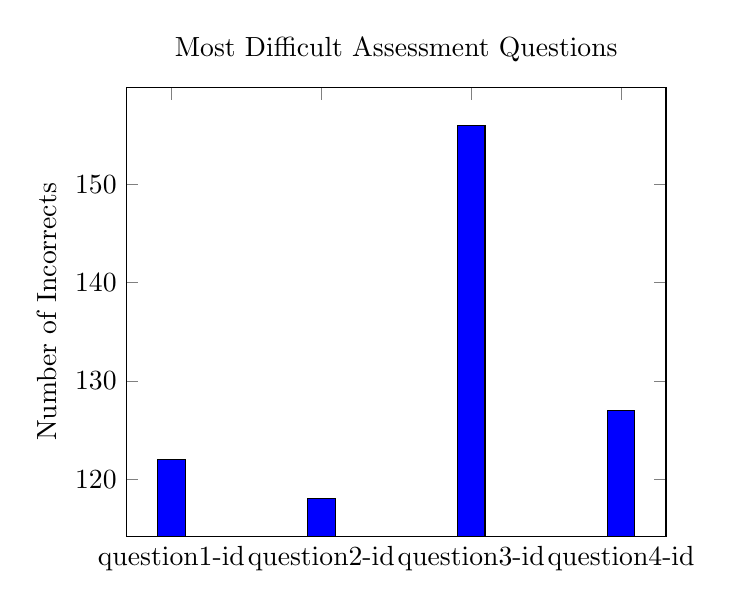
\begin{tikzpicture}
  \begin{axis}[
    title = Most Difficult Assessment Questions,
    ylabel = Number of Incorrects,
    symbolic x coords={question1-id,question2-id,question3-id,question4-id},
    xtick=data]
    \addplot[ybar,fill=blue] coordinates{
      (question1-id,122)
      (question2-id,118)
      (question3-id,156)
      (question4-id,127)
    };
  \end{axis}
\end{tikzpicture}

\subsection{Prototype Improvement Suggestions}
Additional features may be implemented on top of this base
specification but they would require adding aditional values to each
subarray returned by the algorithm. These additional values can be
retrieved via (1) performing metadata lookup within or independently
of the algorithm (2) by utilizing additional xAPI statement paramters
and/or (3) by performing additional computations. The following
examples assume the metadata is contained within each statement
available to the algorithm.

\begin{itemize}
\item Use the name of the activity for the x-axis label instead of
  its id.
  \begin{itemize}
  \item $\$.object.definition.name$
  \item grouping of statements should still happen by
    $\$.object.id$ to ensure an accurate count
  \end{itemize}
\item a tooltip containing contextual information about the question
  such as:
  \begin{itemize}
  \item The question text
    \begin{itemize}
    \item $\$.object.definition.description$
    \end{itemize}
  \item Interaction Type
    \begin{itemize}
    \item $\$.object.definition$ which contains interaction properties
    \end{itemize}
  \item Answer choices
    \begin{itemize}
    \item $\$.object.definition$ which contains interaction properties
    \end{itemize}
  \item Correct answer
    \begin{itemize}
    \item $\$.object.definition$ which contains interaction properties
    \end{itemize}
  \item Most popular incorrect answer
    \begin{itemize}
    \item This would require an extra step of processing and all
      statements would need to utilize interaction properties within
      $\$.object.definition$
    \end{itemize}
  \item average partial credit earned (if applicable)
    \begin{itemize}
    \item $\$.result.score.scaled$
    \item The one potential issue with using scaled score is the
      calculation of scaled is not stricly defined by the xAPI
      specification but is instead up to the authors of the LRP. This
      results in the inability to reliably compare scaled scores across LRPs.
    \item if $\$.result.score.raw$ , $\$.result.score.min$ and
      $\$.result.score.max$ are reported for all questions, it becomes
      possible to reliably compare scores across questions and LRPs.
    \end{itemize}
  \item average number of re-attempts
    \begin{itemize}
    \item this would require additional steps of processing so that
      $\$.actor$ is considered as well
    \item due to the problem of actor unification, ie the same
      person being identified differently across statements, this
      metric may not be accurate.
    \end{itemize}
  \item average time spent on the question
    \begin{itemize}
    \item $\$.result.duration$
    \item this would require additional steps of processing to
      extract the duration and average it.
    \end{itemize}
  \end{itemize}
\item a tooltip containing contextual information about the course
  and/or assessment the question was within
  \begin{itemize}
  \item the instructor for the course
    \begin{itemize}
    \item $\$.context.instructor$
    \end{itemize}
  \item competency associated with the question and/or course
    \begin{itemize}
    \item $\$.context.contextActivities$
    \end{itemize}
  \item metadata about the learning content associated with the
    question such as average time spent engaging with associated
    content before attempting the question.
  \item this would require additional steps of processing to
    retrieve metadata about the content and its usage.
    \begin{itemize}
    \item $\$.context.contextActivities$
    \end{itemize}
  \end{itemize}
\end{itemize}

\end{document}
